    \section*{Теоретическая часть.}

    \begin{figure}[h!]
        \centering
        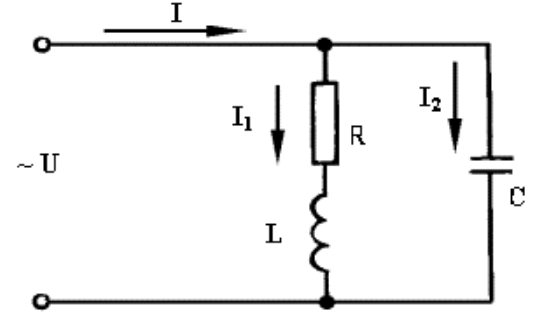
\includegraphics[scale = 0.3]{схема_цепи.png}
        \caption{Схема цепи}
    \end{figure}

    \noindent В этой схеме общим параметром для двух ветвей является напряжение $U$. 
    Первая ветвь -- индуктивная катушка -- обладает активным сопротивлением $R$ и индуктивностью $L$. 
    Результирующее сопротивление $Z_1$ и ток $I_1$ определяются по формуле:

    \begin{equation*}
        Z_1 = \sqrt{R^2 + X_L^2}
    \end{equation*}
    где $X_L = \omega L$.
    \begin{equation*}
        I_1 = \frac{U(t)}{Z_1}
    \end{equation*}

    \noindent Ток в ветви отстает по фазе от напряжения на угол

    \begin{equation*}
        \varphi_1 = \arctan \frac{R}{X_L}
    \end{equation*}

    \begin{figure}[h!]
        \centering
        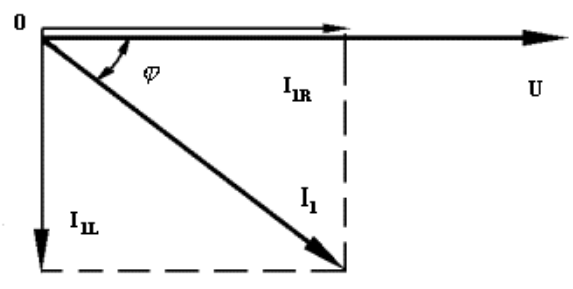
\includegraphics[scale = 0.3]{фазовая_диаграмма1.png}
        \caption{фазовая диаграмма}
    \end{figure}

    \noindent Во вторую ветвь включен конденсатор. Его сопротивление

    \begin{equation*}
        Z_2 = X_C = \frac{1}{\omega L}
    \end{equation*}

    \begin{equation*}
        \frac{U(t)}{Z_2}
    \end{equation*}

    \noindent Этот ток опережает по фазе напряжение на $\frac{\pi}{2}$.
    Для определения тока I в неразветвленной части цепи воспользуемся формулой:

    \begin{equation*}
        I = \sqrt{I_R^2 + (I_L - I_C)^2}
    \end{equation*}

    \begin{figure}[h!]
        \centering
        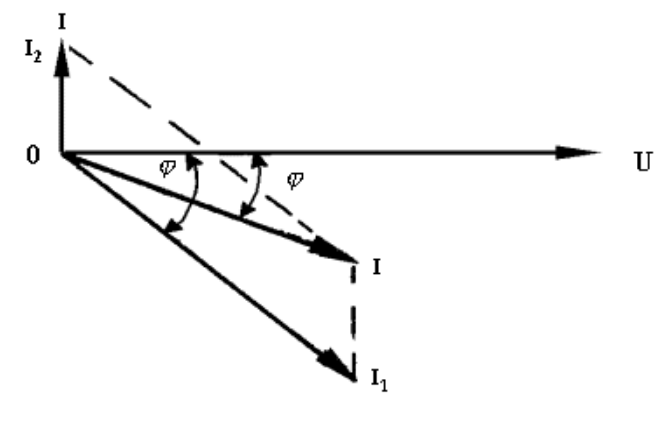
\includegraphics[scale = 0.3]{фазовая_диаграмма2.png}
        \caption{фазовая диаграмма}
    \end{figure}

    \noindent Угол сдвига между током и напряжением обозначим буквой $\theta$.

    \noindent Возможен режим работы схемы, когда $\theta = 0$, 
    т.е. ток в неразветвленной части цепи I будет иметь активный характер. 
    Произойдет это в случае, когда $I_L = I_C$, 
    т.е. при равенстве реактивных составляющих тока в ветвях.

    \begin{figure}[h!]
        \centering
        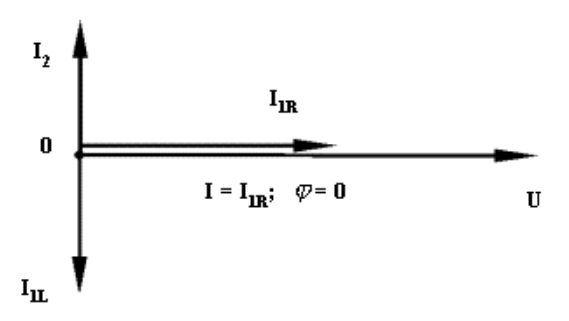
\includegraphics[scale = 0.3]{фазовая_диаграмма3.png}
        \caption{фазовая диаграмма}
    \end{figure}

    \noindent Такой режим называется резонансом токов.

    \noindent Найдем условие, при котором возникает резонанс токов.
    Как видно из фазовой диаграммы:

    \begin{equation*}
        I_2 = I_1 \sin \varphi \Rightarrow
    \end{equation*}

    \begin{equation*}
        \sin \varphi = \frac{\omega L}{\sqrt{R^2 + (\omega L)^2}}
    \end{equation*}

    \begin{equation*}
        \cos \varphi = \frac{R}{\sqrt{R^2 + (\omega L)^2}}
    \end{equation*}

    Таким образом, условие резонанса токов:

    \begin{equation*}
        \omega = \omega_0 = \frac{1}{\sqrt{LC}}
    \end{equation*}

    Вычислим теперь амплитуду полного тока при резонансе.

    \begin{equation*}
        I = I_1 \cos \varphi
    \end{equation*}

    \begin{equation*}
        I = \frac{U_0}{\sqrt{R^2 + (\omega L)^2}} \cdot \frac{R}{\sqrt{R^2 + (\omega L)^2}} \approx \frac{U_0 R C}{L}
    \end{equation*}

    Тогда выразим резонансное напряжение:

    \begin{equation*}
        R_{\text{рез}} = \frac{U_0}{I} = \frac{L}{R C}
    \end{equation*}

    \noindent Отношение резонансного сопративления $R_{\text{рез}}$ контура
    к его активному сопративлению равно квадрату добротности контура.

    \begin{equation*}
        Q^2 = \frac{R_{\text{рез}}}{R}
    \end{equation*}

    \section*{Подготовка.}

    \noindent \textbf{В работе используются:} изучение параллельной цепи переменного тока, наблюдение резонанса токов.
	
	\noindent \textbf{Цель работы:} лабораторный автотрансформатор (ЛАТР),
    разделительный понижающий трансформатор, ёмкость, дроссель с переменной индуктивностью, три амперметра, вольтметр, реостат, электронный осциллограф, омметр, мост переменного тока.
	
    \hfill

    \noindent \textbf{Эксперементальная установка.}

    \noindent Схема экспериментальной установки
    приведена на рисунке. Напряжение от сети (220 В, 50 Гц) с помощью ЛАТРа через понижающий трансформатор Тр подаётся на параллельный
    контур, содержащий конденсатор ($C$ = 120 мкФ) и катушку, индуктивность которой зависит от глубины погружения сердечника. Полный ток
    в цепи измеряется с помощью многопредельного амперметра $A_1$; для измерения токов в $L$ и $C$ ветвях используются два одинаковых амперметра
    $A_2$ и $A_3$; напряжение на контуре контролируется электронным вольтметром V. Последовательно с контуром включён резистор $r$ -- реостат с полным сопротивлением $\simeq 100$ Ом.

    \begin{figure}[h!]
        \centering
        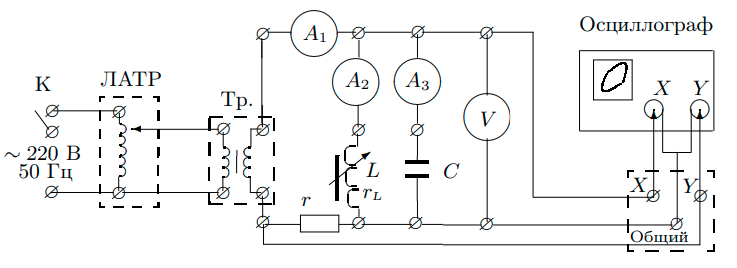
\includegraphics[scale = 0.6]{Схема_эксперементальной_установки.png}
        \caption{}
    \end{figure}

    \hfill

    \noindent Для наблюдения за сдвигом фаз между полным током и напряжением
    на контуре используется осциллограф. Сигнал, пропорциональный току,
    снимается с резистора $r$ и подаётся на вход $Y$ осциллографа. На вход $X$
    подаётся напряжение непосредственно с контура. При наличии сдвига
    фаз между этими напряжениями на экране виден эллипс, а при нулевом
    сдвиге фаз эллипс вырождается в прямую.